%%%%%%%%%%%%%%%%%%%%%%%%%%%%%%%%%%%%%%%%%%%%%%%%%%%%%%%%%%%%%%%%%%%

\chapter {Erstellung von Diagrammen} \label{v:diagramme}

Hier folgen einige kurze Hinweise zur Erstellung von Diagrammen in
den Protokollen des Praktikums.

\section{Allgemeines}

Die meisten Auswertungen in der Physik werden heute mit sehr
umfangreichen Programmpaketen durchgef"uhrt, die auch gleichzeitig
eine komfortable Diagrammerstellung erlauben. Dennoch kann es
vorkommen, dass man eine einfache Auswertung sehr viel schneller
und mit guter Genauigkeit auch auf konventionellem Wege auf
Millimeterpapier oder Logarithmenpapier ausf"uhren kann. Zudem sind
die hier folgenden Hinweise auch sehr n"utzlich, wenn man
Computerprogramme zur Diagrammerstellung verwendet.

Manuelle Diagramme sind grunds"atzlich immer auf Millimeter- oder
Logarithmenpapier anzufertigen. Bei Computerprogrammen kann auf dies
verzichtet werden, dennoch sollte man auch hier auf eine leichte
Ablesbarkeit der Daten achten.

\section{Achsen}


\begin{enumerate}
    \item Wahl der Achsen: Die unabh"angige (die eingestellte)
    Variable sollte auf der waagerechten Achse, der "`x-Achse"'
    (Abszisse\index{Abszisse}), aufgetragen werden. Die abh"angige (die
    gemessene) Variable sollte auf der vertikalen Achse, der "`y-Achse"'
    (Ordinate\index{Ordinate}), aufgetragen werden.
    \item Achseneinteilung: Die Achseneinteilung sollte so gew"ahlt
    werden, das die Werte eines Datenpunktes einfach und schnell
    ermittelt werden k"onnen. Drei Einheiten einer Gr"o{\ss}e auf einem Zentimeter einzuzeichnen macht also nicht viel Sinn.
    \item Nullpunktsunterdr"uckung: Der Wertebereich der Achsen
    sollte so gew"ahlt werden, dass ein m"oglichst gro"ser Bereich
    ausgef"ullt wird (mindestens 75\% des Diagrammbereiches). Hierbei kann der Nullpunkt
    unterdr"uckt werden, wenn kein triftiger Grund dagegen
    spricht. Das bedeutet, dass die Einheiten auf Abszisse und Ordinate nicht unbedingt bei x=y=0 anfangen m"ussen. Dies gilt auch f"ur logarithmische Skalen.
    \item Achsen sind zu beschriften! Was ist aufgetragen?
    Zahlenwerte sind anzugeben. Einheiten sind unverzichtbar.
    \item Bei logarithmierten Werten ist die Angabe der Einheit problematisch,
     da der Logarithmus im Argument keine Einheit haben darf. Hier teilt man die
     Messwerte einfach durch die Einheit und erh"alt so reine Zahlenwert. Dies ist
     dann auch so anzugeben.
\end{enumerate}

\section{Datenpunkte und Fehlerbalken}

\begin{itemize}
    \item Symbole: Die Messpunkte sollten durch deutliche Symbole
    gekennzeichnet werden. "Ublich sind zum Beispiel: $ \square \blacksquare
    \blacktriangle \blacktriangledown \lozenge \blacklozenge \vartriangle
    \triangledown \bullet \bigcirc \circ \ast \star$.
    \item Unterschiedliche Messreihen sollten auch durch
    unterschiedliche Symbole gekennzeichnet werden. Auf eine
    eindeutige Legende ist zu achten. Farbe kann hier sehr
    n"utzlich sein, doch diese geht leider beim Kopieren verloren.
    \item Fehlerbalken: Normalerweise sind alle Messpunkte mit
    Fehlerbalken zu versehen, deren L"ange der Gr"o"se des (1$\sigma$-)Fehlers
    auf den jeweiligen Messwert entspricht. Dabei kann es notwendig sein, in
    den verschiedenen Achsrichtungen unterschiedlich gro"se
    Fehlerbalken zu verwenden.
\end{itemize}

\section{Kurven und Verbindungslinien}


\begin{itemize}
    \item Eine durchgezogene Kurve kann die Lesbarkeit einer
    Darstellung deutlich erh"ohen. Dennoch sollte dies mit Bedacht
    angewendet werden.
    \item In allen F"allen des Praktikums sind "`glatte"' Kurven zu
    erwarten. Zumeist ist der funktionale Zusammenhang der
    Messdaten auch durch die Theorie schon bekannt. Im Allgemeinen
    sollte eine Kurve m"oglichst wenig Wendepunkte haben.
    \item Es ist nicht zwingend erforderlich, dass die
    durchgezogene Kurve alle, oder "uberhaupt, Messpunkte trifft.
    Endpunkte sind meist weniger genau und m"ussen nicht unbedingt
    getroffen werden. Das einfache lineare Verbinden der
    Messpunkte durch eine
    "`Zick-Zack-Kurve"' ist physikalisch kompletter Unsinn und
    sollte unterlassen werden.
    \item Die Kurve sollte m"oglichst dicht an den Messpunkten
    liegen (Minimierung der Fehlerquadrate). Die eingezeichneten
    Fehlerbalken k"onnen hier eine gute Hilfe sein. Zudem ist das
    Auge ein sehr guter "`Computer"' f"ur die Ausgleichskurve.
    \item Im Wesentlichen sollte die Kurve die Messpunkte
    halbieren, d.h. eine H"alfte der Punkte "uber der Kurve, die
    andere darunter. Das gilt sinngem"a"s auch f"ur Teilst"ucke.
    \item An Regressionsgeraden sind auch die Ergebnisse der
    Regression mit den richtigen Einheiten anzugeben.
    \item Bei Ermittlung des Fehlers "uber Grenzgeraden, sind auch
    diese in der Zeichnung anzudeuten.
\end{itemize}

Als Beispiel f"ur die Diagrammerstellung sind in
Bild~\ref{a:graph_beisp} zwei typische Diagramme aufgef"uhrt.
%
\begin{figure}[htb]
  \centering
  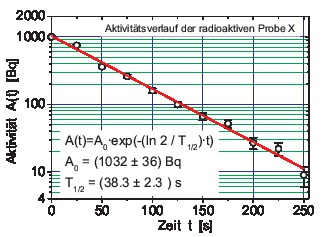
\includegraphics[width=6.5cm]{00_einl/graph_expzerf}
  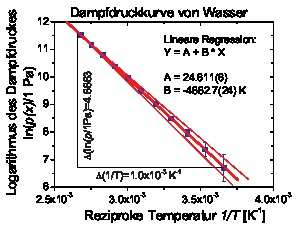
\includegraphics[width=6.5cm]{00_einl/graph_dampf}
  \caption[Diagramm-Beispiele]{\label{a:graph_beisp}Beispiele f"ur grafische Auftragungen
   zu Messwerten und Auswertungen:
  a) (links) Halblogarithmische Darstellung des exponentiellen Zerfalls;
  b) (rechts) Arrheniusplot der Dampfdruckkurve von Wasser. }
\end{figure}
%
Die Aktivit"atskurve wird
halblogarithmisch\index{Logarithmenpapier!halblogarithmisch}
aufgetragen, d.h. die Zeit normal (linear) als x-Achse, w"ahrend
die Aktivit"at logarithmisch
(Logarithmenpapier\index{Logarithmenpapier}) aufgetragen
wird.\footnote{Es erfolgt keine Umrechnung der Messwerte, die
Skalenteilung ist logarithmisch, genauer gesagt
halblogarithmisch.} Dies hat zur Folge, dass aus der
Exponentialfunktion eine lineare Funktion wird:
%
\begin{equation}\label{e:bsp_exp}
    A(t)=A_0 \cdot \exp(-\lambda t) \Longrightarrow \ln(A(t)) =
    \ln(A_0) - \lambda t
\end{equation}
%
Die Zerfallskonstante $\lambda$ kann dann aus der Steigung $m$ der
sich ergebenden Geraden ermittelt werden, woraus dann die
Halbwertszeit folgt. Man beachte die unterschiedliche L"ange der
Fehlerbalken. F"ur viele Skalengesetze und stark streuende Messwerte,
oder wenn man den Zusammenhang nicht genau kennt, verwendet man die
doppeltlogarithmische
Auftragung\index{Logarithmenpapier!doppeltlogarithmisch}, die f"ur
fast alle beliebigen Messungen eine Gerade entstehen l"asst.

In Bild~\ref{a:graph_beisp}b) ist ein Arrheniusplot des Dampfdruckes
von Wasser aufgetragen. Hier werden die Messwerte (in Pa) vor dem
Auftragen durch ihren Logarithmus ersetzt. Da das Argument des
Logarithmus keine Einheit enthalten kann, behilft man sich, indem
man durch die Einheit dividiert (d.h. diese "`Basiseinheit"' muss
auch im Diagramm mit angegeben werden). Durch die Auftragung der
logarithmierten Messwerte gegen die reziproke Temperatur erh"alt man
eine Gerade
%
\begin{equation}\label{e:bsp_dampf}
    p(T) = p_0 \cdot \exp\left( - \frac{\Lambda}{RT} \right) \Rightarrow
    \ln\left( p(T) \right) = \ln(p_0) - \frac{\Lambda}{R} \cdot
    \frac{1}{T} \, ,
\end{equation}
%
aus deren Steigung die Verdampfungsenthalpie $\Lambda$ berechnet
werden kann. Das Steigungsdreieck ist eingezeichnet und die Steigung
ergibt sich zu
$m=\frac{\mathrm{4.883}}{\mathrm{1\cdot 10^{-3}\, K^{-1}}}=\mathrm{4883~K}$.\footnote{Bitte
beachten Sie, dass die Steigung nat"urlich eine Einheit hat, die
angegeben werden muss.} Mit der allgemeinen Gaskonstanten
$R=\mathrm{8.3145\,J \, mol^{-1} \, K^{-1}}$ ergibt sich die
Verdampfungsw"arme zu $\Lambda=m \cdot R = \mathrm{40597\,J \,mol^{-1}}$ mit einem Fehler von $\Delta \Lambda = \mathrm{20\,J \,mol^{-1}}$.
